\documentclass[1p]{elsarticle_modified}
%\bibliographystyle{elsarticle-num}

%\usepackage[colorlinks]{hyperref}
%\usepackage{abbrmath_seonhwa} %\Abb, \Ascr, \Acal ,\Abf, \Afrak
\usepackage{amsfonts}
\usepackage{amssymb}
\usepackage{amsmath}
\usepackage{amsthm}
\usepackage{scalefnt}
\usepackage{amsbsy}
\usepackage{kotex}
\usepackage{caption}
\usepackage{subfig}
\usepackage{color}
\usepackage{graphicx}
\usepackage{xcolor} %% white, black, red, green, blue, cyan, magenta, yellow
\usepackage{float}
\usepackage{setspace}
\usepackage{hyperref}

\usepackage{tikz}
\usetikzlibrary{arrows}

\usepackage{multirow}
\usepackage{array} % fixed length table
\usepackage{hhline}

%%%%%%%%%%%%%%%%%%%%%
\makeatletter
\renewcommand*\env@matrix[1][\arraystretch]{%
	\edef\arraystretch{#1}%
	\hskip -\arraycolsep
	\let\@ifnextchar\new@ifnextchar
	\array{*\c@MaxMatrixCols c}}
\makeatother %https://tex.stackexchange.com/questions/14071/how-can-i-increase-the-line-spacing-in-a-matrix
%%%%%%%%%%%%%%%

\usepackage[normalem]{ulem}

\newcommand{\msout}[1]{\ifmmode\text{\sout{\ensuremath{#1}}}\else\sout{#1}\fi}
%SOURCE: \msout is \stkout macro in https://tex.stackexchange.com/questions/20609/strikeout-in-math-mode

\newcommand{\cancel}[1]{
	\ifmmode
	{\color{red}\msout{#1}}
	\else
	{\color{red}\sout{#1}}
	\fi
}

\newcommand{\add}[1]{
	{\color{blue}\uwave{#1}}
}

\newcommand{\replace}[2]{
	\ifmmode
	{\color{red}\msout{#1}}{\color{blue}\uwave{#2}}
	\else
	{\color{red}\sout{#1}}{\color{blue}\uwave{#2}}
	\fi
}

\newcommand{\Sol}{\mathcal{S}} %segment
\newcommand{\D}{D} %diagram
\newcommand{\A}{\mathcal{A}} %arc


%%%%%%%%%%%%%%%%%%%%%%%%%%%%%5 test

\def\sl{\operatorname{\textup{SL}}(2,\Cbb)}
\def\psl{\operatorname{\textup{PSL}}(2,\Cbb)}
\def\quan{\mkern 1mu \triangleright \mkern 1mu}

\theoremstyle{definition}
\newtheorem{thm}{Theorem}[section]
\newtheorem{prop}[thm]{Proposition}
\newtheorem{lem}[thm]{Lemma}
\newtheorem{ques}[thm]{Question}
\newtheorem{cor}[thm]{Corollary}
\newtheorem{defn}[thm]{Definition}
\newtheorem{exam}[thm]{Example}
\newtheorem{rmk}[thm]{Remark}
\newtheorem{alg}[thm]{Algorithm}

\newcommand{\I}{\sqrt{-1}}
\begin{document}

%\begin{frontmatter}
%
%\title{Boundary parabolic representations of knots up to 8 crossings}
%
%%% Group authors per affiliation:
%\author{Yunhi Cho} 
%\address{Department of Mathematics, University of Seoul, Seoul, Korea}
%\ead{yhcho@uos.ac.kr}
%
%
%\author{Seonhwa Kim} %\fnref{s_kim}}
%\address{Center for Geometry and Physics, Institute for Basic Science, Pohang, 37673, Korea}
%\ead{ryeona17@ibs.re.kr}
%
%\author{Hyuk Kim}
%\address{Department of Mathematical Sciences, Seoul National University, Seoul 08826, Korea}
%\ead{hyukkim@snu.ac.kr}
%
%\author{Seokbeom Yoon}
%\address{Department of Mathematical Sciences, Seoul National University, Seoul, 08826,  Korea}
%\ead{sbyoon15@snu.ac.kr}
%
%\begin{abstract}
%We find all boundary parabolic representation of knots up to 8 crossings.
%
%\end{abstract}
%\begin{keyword}
%    \MSC[2010] 57M25 
%\end{keyword}
%
%\end{frontmatter}

%\linenumbers
%\tableofcontents
%
\newcommand\colored[1]{\textcolor{white}{\rule[-0.35ex]{0.8em}{1.4ex}}\kern-0.8em\color{red} #1}%
%\newcommand\colored[1]{\textcolor{white}{ #1}\kern-2.17ex	\textcolor{white}{ #1}\kern-1.81ex	\textcolor{white}{ #1}\kern-2.15ex\color{red}#1	}

{\Large $\underline{12a_{0594}~(K12a_{0594})}$}

\setlength{\tabcolsep}{10pt}
\renewcommand{\arraystretch}{1.6}
\vspace{1cm}\begin{tabular}{m{100pt}>{\centering\arraybackslash}m{274pt}}
\multirow{5}{120pt}{
	\centering
	\includegraphics[width=112pt]{../../../GIT/diagram.site/Diagrams/png/1395_12a_0594.png}\\
\ \ \ A knot diagram\footnotemark}&
\allowdisplaybreaks
\textbf{Linearized knot diagam} \\
\cline{2-2}
 &
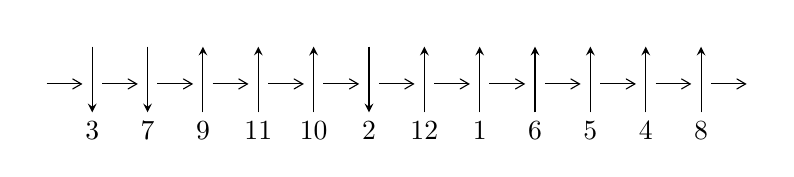
\begin{tikzpicture}[x=20pt, y=17pt]
	% nodes
	\node (C0) at (0, 0) {};
	\node (C1) at (1, 0) {};
	\node (C1U) at (1, +1) {};
	\node (C1D) at (1, -1) {3};

	\node (C2) at (2, 0) {};
	\node (C2U) at (2, +1) {};
	\node (C2D) at (2, -1) {7};

	\node (C3) at (3, 0) {};
	\node (C3U) at (3, +1) {};
	\node (C3D) at (3, -1) {9};

	\node (C4) at (4, 0) {};
	\node (C4U) at (4, +1) {};
	\node (C4D) at (4, -1) {11};

	\node (C5) at (5, 0) {};
	\node (C5U) at (5, +1) {};
	\node (C5D) at (5, -1) {10};

	\node (C6) at (6, 0) {};
	\node (C6U) at (6, +1) {};
	\node (C6D) at (6, -1) {2};

	\node (C7) at (7, 0) {};
	\node (C7U) at (7, +1) {};
	\node (C7D) at (7, -1) {12};

	\node (C8) at (8, 0) {};
	\node (C8U) at (8, +1) {};
	\node (C8D) at (8, -1) {1};

	\node (C9) at (9, 0) {};
	\node (C9U) at (9, +1) {};
	\node (C9D) at (9, -1) {6};

	\node (C10) at (10, 0) {};
	\node (C10U) at (10, +1) {};
	\node (C10D) at (10, -1) {5};

	\node (C11) at (11, 0) {};
	\node (C11U) at (11, +1) {};
	\node (C11D) at (11, -1) {4};

	\node (C12) at (12, 0) {};
	\node (C12U) at (12, +1) {};
	\node (C12D) at (12, -1) {8};
	\node (C13) at (13, 0) {};

	% arrows
	\draw[->,>={angle 60}]
	(C0) edge (C1) (C1) edge (C2) (C2) edge (C3) (C3) edge (C4) (C4) edge (C5) (C5) edge (C6) (C6) edge (C7) (C7) edge (C8) (C8) edge (C9) (C9) edge (C10) (C10) edge (C11) (C11) edge (C12) (C12) edge (C13) ;	\draw[->,>=stealth]
	(C1U) edge (C1D) (C2U) edge (C2D) (C3D) edge (C3U) (C4D) edge (C4U) (C5D) edge (C5U) (C6U) edge (C6D) (C7D) edge (C7U) (C8D) edge (C8U) (C9D) edge (C9U) (C10D) edge (C10U) (C11D) edge (C11U) (C12D) edge (C12U) ;
	\end{tikzpicture} \\
\hhline{~~} \\& 
\textbf{Solving Sequence} \\ \cline{2-2} 
 &
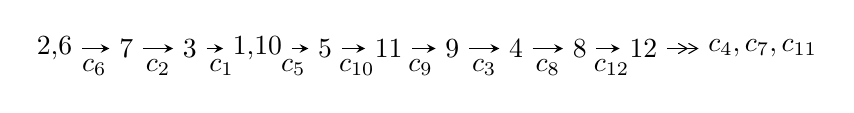
\begin{tikzpicture}[x=23pt, y=7pt]
	% node
	\node (A0) at (-1/8, 0) {2,6};
	\node (A1) at (1, 0) {7};
	\node (A2) at (2, 0) {3};
	\node (A3) at (49/16, 0) {1,10};
	\node (A4) at (33/8, 0) {5};
	\node (A5) at (41/8, 0) {11};
	\node (A6) at (49/8, 0) {9};
	\node (A7) at (57/8, 0) {4};
	\node (A8) at (65/8, 0) {8};
	\node (A9) at (73/8, 0) {12};
	\node (C1) at (1/2, -1) {$c_{6}$};
	\node (C2) at (3/2, -1) {$c_{2}$};
	\node (C3) at (5/2, -1) {$c_{1}$};
	\node (C4) at (29/8, -1) {$c_{5}$};
	\node (C5) at (37/8, -1) {$c_{10}$};
	\node (C6) at (45/8, -1) {$c_{9}$};
	\node (C7) at (53/8, -1) {$c_{3}$};
	\node (C8) at (61/8, -1) {$c_{8}$};
	\node (C9) at (69/8, -1) {$c_{12}$};
	\node (A10) at (11, 0) {$c_{4},c_{7},c_{11}$};

	% edge
	\draw[->,>=stealth]	
	(A0) edge (A1) (A1) edge (A2) (A2) edge (A3) (A3) edge (A4) (A4) edge (A5) (A5) edge (A6) (A6) edge (A7) (A7) edge (A8) (A8) edge (A9) ;
	\draw[->>,>={angle 60}]	
	(A9) edge (A10);
\end{tikzpicture} \\ 

\end{tabular} \\

\footnotetext{
The image of knot diagram is generated by the software ``\textbf{Draw programme}" developed by Andrew Bartholomew(\url{http://www.layer8.co.uk/maths/draw/index.htm\#Running-draw}), where we modified some parts for our purpose(\url{https://github.com/CATsTAILs/LinksPainter}).
}\phantom \\ \newline 
\centering \textbf{Ideals for irreducible components\footnotemark of $X_{\text{par}}$} 
 
\begin{align*}
I^u_{1}&=\langle 
-278579575 u^{38}+801007023 u^{37}+\cdots+960147928 b+4668885888,\\
\phantom{I^u_{1}}&\phantom{= \langle  }-506726616 u^{38}+1536859595 u^{37}+\cdots+960147928 a+7944281003,\;u^{39}-2 u^{38}+\cdots+13 u-8\rangle \\
I^u_{2}&=\langle 
- u^6+2 u^4- u^2+b,\;- u^6+u^4+a+1,\\
\phantom{I^u_{2}}&\phantom{= \langle  }u^{15}-5 u^{13}+u^{12}+10 u^{11}-4 u^{10}-10 u^9+6 u^8+5 u^7-5 u^6- u^5+3 u^4+u^3- u^2- u+1\rangle \\
I^u_{3}&=\langle 
2 b- a+1,\;a^2-2 a+13,\;u+1\rangle \\
I^u_{4}&=\langle 
2 b- a+1,\;a^2-2 a+5,\;u-1\rangle \\
I^u_{5}&=\langle 
b,\;a-1,\;u+1\rangle \\
\\
\end{align*}
\raggedright * 5 irreducible components of $\dim_{\mathbb{C}}=0$, with total 59 representations.\\
\footnotetext{All coefficients of polynomials are rational numbers. But the coefficients are sometimes approximated in decimal forms when there is not enough margin.}
\newpage
\renewcommand{\arraystretch}{1}
\centering \section*{I. $I^u_{1}= \langle -2.79\times10^{8} u^{38}+8.01\times10^{8} u^{37}+\cdots+9.60\times10^{8} b+4.67\times10^{9},\;-5.07\times10^{8} u^{38}+1.54\times10^{9} u^{37}+\cdots+9.60\times10^{8} a+7.94\times10^{9},\;u^{39}-2 u^{38}+\cdots+13 u-8 \rangle$}
\flushleft \textbf{(i) Arc colorings}\\
\begin{tabular}{m{7pt} m{180pt} m{7pt} m{180pt} }
\flushright $a_{2}=$&$\begin{pmatrix}0\\u\end{pmatrix}$ \\
\flushright $a_{6}=$&$\begin{pmatrix}1\\0\end{pmatrix}$ \\
\flushright $a_{7}=$&$\begin{pmatrix}1\\u^2\end{pmatrix}$ \\
\flushright $a_{3}=$&$\begin{pmatrix}- u\\- u^3+u\end{pmatrix}$ \\
\flushright $a_{1}=$&$\begin{pmatrix}u^3\\u^5- u^3+u\end{pmatrix}$ \\
\flushright $a_{10}=$&$\begin{pmatrix}0.527759 u^{38}-1.60065 u^{37}+\cdots+10.7329 u-8.27402\\0.290142 u^{38}-0.834254 u^{37}+\cdots+7.56410 u-4.86267\end{pmatrix}$ \\
\flushright $a_{5}=$&$\begin{pmatrix}0.785150 u^{38}-0.610681 u^{37}+\cdots+11.4919 u-1.16835\\0.354400 u^{38}-0.130647 u^{37}+\cdots+2.97397 u+2.89166\end{pmatrix}$ \\
\flushright $a_{11}=$&$\begin{pmatrix}-0.848153 u^{38}+2.71323 u^{37}+\cdots-15.2658 u+5.19809\\-0.487224 u^{38}+1.44307 u^{37}+\cdots-12.6317 u+7.27384\end{pmatrix}$ \\
\flushright $a_{9}=$&$\begin{pmatrix}0.237617 u^{38}-0.766395 u^{37}+\cdots+3.16882 u-3.41134\\0.290142 u^{38}-0.834254 u^{37}+\cdots+7.56410 u-4.86267\end{pmatrix}$ \\
\flushright $a_{4}=$&$\begin{pmatrix}0.150856 u^{38}+0.0217381 u^{37}+\cdots-17.3547 u+9.46883\\0.170865 u^{38}-0.242768 u^{37}+\cdots-12.7382 u+5.24191\end{pmatrix}$ \\
\flushright $a_{8}=$&$\begin{pmatrix}0.508134 u^{38}-1.24630 u^{37}+\cdots+5.04688 u-6.94472\\0.466487 u^{38}-1.22328 u^{37}+\cdots+7.11369 u-4.38047\end{pmatrix}$ \\
\flushright $a_{12}=$&$\begin{pmatrix}0.546702 u^{38}-2.31337 u^{37}+\cdots+5.56221 u-1.82639\\0.230030 u^{38}-1.40951 u^{37}+\cdots+12.5505 u-4.06507\end{pmatrix}$\\&\end{tabular}
\flushleft \textbf{(ii) Obstruction class $= -1$}\\~\\
\flushleft \textbf{(iii) Cusp Shapes $= \frac{1009740537}{480073964} u^{38}-\frac{2449057759}{480073964} u^{37}+\cdots+\frac{13839136571}{480073964} u+\frac{1544450212}{120018491}$}\\~\\
\newpage\renewcommand{\arraystretch}{1}
\flushleft \textbf{(iv) u-Polynomials at the component}\newline \\
\begin{tabular}{m{50pt}|m{274pt}}
Crossings & \hspace{64pt}u-Polynomials at each crossing \\
\hline $$\begin{aligned}c_{1}\end{aligned}$$&$\begin{aligned}
&u^{39}+16 u^{38}+\cdots+841 u+64
\end{aligned}$\\
\hline $$\begin{aligned}c_{2},c_{6}\end{aligned}$$&$\begin{aligned}
&u^{39}-2 u^{38}+\cdots+13 u-8
\end{aligned}$\\
\hline $$\begin{aligned}c_{3}\end{aligned}$$&$\begin{aligned}
&u^{39}+2 u^{38}+\cdots-434 u-82
\end{aligned}$\\
\hline $$\begin{aligned}c_{4},c_{5},c_{9}\\c_{10},c_{11}\end{aligned}$$&$\begin{aligned}
&u^{39}+2 u^{38}+\cdots-6 u-2
\end{aligned}$\\
\hline $$\begin{aligned}c_{7},c_{8},c_{12}\end{aligned}$$&$\begin{aligned}
&u^{39}+2 u^{38}+\cdots-3 u-8
\end{aligned}$\\
\hline
\end{tabular}\\~\\
\newpage\renewcommand{\arraystretch}{1}
\flushleft \textbf{(v) Riley Polynomials at the component}\newline \\
\begin{tabular}{m{50pt}|m{274pt}}
Crossings & \hspace{64pt}Riley Polynomials at each crossing \\
\hline $$\begin{aligned}c_{1}\end{aligned}$$&$\begin{aligned}
&y^{39}+20 y^{38}+\cdots+20945 y-4096
\end{aligned}$\\
\hline $$\begin{aligned}c_{2},c_{6}\end{aligned}$$&$\begin{aligned}
&y^{39}-16 y^{38}+\cdots+841 y-64
\end{aligned}$\\
\hline $$\begin{aligned}c_{3}\end{aligned}$$&$\begin{aligned}
&y^{39}+2 y^{38}+\cdots-278552 y-6724
\end{aligned}$\\
\hline $$\begin{aligned}c_{4},c_{5},c_{9}\\c_{10},c_{11}\end{aligned}$$&$\begin{aligned}
&y^{39}+50 y^{38}+\cdots+8 y-4
\end{aligned}$\\
\hline $$\begin{aligned}c_{7},c_{8},c_{12}\end{aligned}$$&$\begin{aligned}
&y^{39}-40 y^{38}+\cdots-535 y-64
\end{aligned}$\\
\hline
\end{tabular}\\~\\
\newpage\flushleft \textbf{(vi) Complex Volumes and Cusp Shapes}
$$\begin{array}{c|c|c}  
\text{Solutions to }I^u_{1}& \I (\text{vol} + \sqrt{-1}CS) & \text{Cusp shape}\\
 \hline 
\begin{aligned}
u &= \phantom{-}0.510187 + 0.854260 I \\
a &= \phantom{-}0.459599 + 0.050441 I \\
b &= -0.601563 - 0.109572 I\end{aligned}
 & \phantom{-}7.19513 + 1.98650 I & \phantom{-}12.18743 - 1.52305 I \\ \hline\begin{aligned}
u &= \phantom{-}0.510187 - 0.854260 I \\
a &= \phantom{-}0.459599 - 0.050441 I \\
b &= -0.601563 + 0.109572 I\end{aligned}
 & \phantom{-}7.19513 - 1.98650 I & \phantom{-}12.18743 + 1.52305 I \\ \hline\begin{aligned}
u &= -0.622477 + 0.793703 I \\
a &= \phantom{-}0.715601 - 0.679477 I \\
b &= -0.417743 - 0.676425 I\end{aligned}
 & \phantom{-}5.47691 + 1.45533 I & \phantom{-}8.53847 - 4.19348 I \\ \hline\begin{aligned}
u &= -0.622477 - 0.793703 I \\
a &= \phantom{-}0.715601 + 0.679477 I \\
b &= -0.417743 + 0.676425 I\end{aligned}
 & \phantom{-}5.47691 - 1.45533 I & \phantom{-}8.53847 + 4.19348 I \\ \hline\begin{aligned}
u &= \phantom{-}0.340675 + 0.952778 I \\
a &= \phantom{-}0.461846 - 1.211810 I \\
b &= -0.09622 - 1.69407 I\end{aligned}
 & -5.17058 + 7.10896 I & \phantom{-}5.57947 - 3.18452 I \\ \hline\begin{aligned}
u &= \phantom{-}0.340675 - 0.952778 I \\
a &= \phantom{-}0.461846 + 1.211810 I \\
b &= -0.09622 + 1.69407 I\end{aligned}
 & -5.17058 - 7.10896 I & \phantom{-}5.57947 + 3.18452 I \\ \hline\begin{aligned}
u &= -0.409576 + 0.898054 I \\
a &= \phantom{-}0.444383 + 0.626707 I \\
b &= -0.372437 + 0.928150 I\end{aligned}
 & \phantom{-}4.02432 - 5.28034 I & \phantom{-}7.11448 + 4.34651 I \\ \hline\begin{aligned}
u &= -0.409576 - 0.898054 I \\
a &= \phantom{-}0.444383 - 0.626707 I \\
b &= -0.372437 - 0.928150 I\end{aligned}
 & \phantom{-}4.02432 + 5.28034 I & \phantom{-}7.11448 - 4.34651 I \\ \hline\begin{aligned}
u &= -0.893825 + 0.408631 I \\
a &= \phantom{-}0.56327 - 3.33333 I \\
b &= \phantom{-}0.02030 - 1.76094 I\end{aligned}
 & -12.19790 + 1.67763 I & \phantom{-}3.69120 - 4.54232 I \\ \hline\begin{aligned}
u &= -0.893825 - 0.408631 I \\
a &= \phantom{-}0.56327 + 3.33333 I \\
b &= \phantom{-}0.02030 + 1.76094 I\end{aligned}
 & -12.19790 - 1.67763 I & \phantom{-}3.69120 + 4.54232 I\\
 \hline 
 \end{array}$$\newpage$$\begin{array}{c|c|c}  
\text{Solutions to }I^u_{1}& \I (\text{vol} + \sqrt{-1}CS) & \text{Cusp shape}\\
 \hline 
\begin{aligned}
u &= \phantom{-}0.880857 + 0.533899 I \\
a &= \phantom{-}0.46350 + 1.87403 I \\
b &= \phantom{-}0.098417 + 1.194680 I\end{aligned}
 & -1.54593 - 2.15130 I & \phantom{-}4.04314 + 3.05891 I \\ \hline\begin{aligned}
u &= \phantom{-}0.880857 - 0.533899 I \\
a &= \phantom{-}0.46350 - 1.87403 I \\
b &= \phantom{-}0.098417 - 1.194680 I\end{aligned}
 & -1.54593 + 2.15130 I & \phantom{-}4.04314 - 3.05891 I \\ \hline\begin{aligned}
u &= -0.892947 + 0.364874 I \\
a &= -0.098814 + 0.170736 I \\
b &= -0.264285 + 0.451533 I\end{aligned}
 & -1.36259 + 1.28896 I & \phantom{-}1.24891 - 0.92411 I \\ \hline\begin{aligned}
u &= -0.892947 - 0.364874 I \\
a &= -0.098814 - 0.170736 I \\
b &= -0.264285 - 0.451533 I\end{aligned}
 & -1.36259 - 1.28896 I & \phantom{-}1.24891 + 0.92411 I \\ \hline\begin{aligned}
u &= \phantom{-}1.073090 + 0.243180 I \\
a &= -0.20763 - 1.90178 I \\
b &= -0.131098 - 1.030410 I\end{aligned}
 & -5.77927 - 0.03027 I & -4.62865 - 0.08924 I \\ \hline\begin{aligned}
u &= \phantom{-}1.073090 - 0.243180 I \\
a &= -0.20763 + 1.90178 I \\
b &= -0.131098 + 1.030410 I\end{aligned}
 & -5.77927 + 0.03027 I & -4.62865 + 0.08924 I \\ \hline\begin{aligned}
u &= \phantom{-}0.980860 + 0.516874 I \\
a &= \phantom{-}0.601891 + 0.724041 I \\
b &= -0.513688 + 0.161476 I\end{aligned}
 & -0.27159 - 4.03311 I & \phantom{-}6.10073 + 7.35963 I \\ \hline\begin{aligned}
u &= \phantom{-}0.980860 - 0.516874 I \\
a &= \phantom{-}0.601891 - 0.724041 I \\
b &= -0.513688 - 0.161476 I\end{aligned}
 & -0.27159 + 4.03311 I & \phantom{-}6.10073 - 7.35963 I \\ \hline\begin{aligned}
u &= \phantom{-}0.807984 + 0.807298 I \\
a &= \phantom{-}0.93590 + 1.21554 I \\
b &= -0.03886 + 1.59336 I\end{aligned}
 & -2.08218 - 2.94056 I & \phantom{-}6.18654 + 2.75292 I \\ \hline\begin{aligned}
u &= \phantom{-}0.807984 - 0.807298 I \\
a &= \phantom{-}0.93590 - 1.21554 I \\
b &= -0.03886 - 1.59336 I\end{aligned}
 & -2.08218 + 2.94056 I & \phantom{-}6.18654 - 2.75292 I\\
 \hline 
 \end{array}$$\newpage$$\begin{array}{c|c|c}  
\text{Solutions to }I^u_{1}& \I (\text{vol} + \sqrt{-1}CS) & \text{Cusp shape}\\
 \hline 
\begin{aligned}
u &= \phantom{-}0.587388 + 0.621753 I \\
a &= -0.417391 - 0.020298 I \\
b &= -0.01628 - 1.67009 I\end{aligned}
 & -9.77106 - 1.29915 I & \phantom{-}3.64577 + 3.61671 I \\ \hline\begin{aligned}
u &= \phantom{-}0.587388 - 0.621753 I \\
a &= -0.417391 + 0.020298 I \\
b &= -0.01628 + 1.67009 I\end{aligned}
 & -9.77106 + 1.29915 I & \phantom{-}3.64577 - 3.61671 I \\ \hline\begin{aligned}
u &= -1.153580 + 0.222471 I \\
a &= -0.20810 + 3.24218 I \\
b &= -0.03306 + 1.72517 I\end{aligned}
 & -15.6341 - 0.6387 I & -4.65488 - 0.03706 I \\ \hline\begin{aligned}
u &= -1.153580 - 0.222471 I \\
a &= -0.20810 - 3.24218 I \\
b &= -0.03306 - 1.72517 I\end{aligned}
 & -15.6341 + 0.6387 I & -4.65488 + 0.03706 I \\ \hline\begin{aligned}
u &= -1.063930 + 0.555566 I \\
a &= \phantom{-}1.47957 - 1.38271 I \\
b &= -0.310928 - 0.963275 I\end{aligned}
 & -3.72446 + 6.84807 I & \phantom{-}0.27874 - 7.93372 I \\ \hline\begin{aligned}
u &= -1.063930 - 0.555566 I \\
a &= \phantom{-}1.47957 + 1.38271 I \\
b &= -0.310928 + 0.963275 I\end{aligned}
 & -3.72446 - 6.84807 I & \phantom{-}0.27874 + 7.93372 I \\ \hline\begin{aligned}
u &= -1.008430 + 0.658829 I \\
a &= \phantom{-}0.103228 - 0.321231 I \\
b &= \phantom{-}0.472850 - 0.562157 I\end{aligned}
 & \phantom{-}4.30632 + 4.00074 I & \phantom{-}7.24813 - 1.07966 I \\ \hline\begin{aligned}
u &= -1.008430 - 0.658829 I \\
a &= \phantom{-}0.103228 + 0.321231 I \\
b &= \phantom{-}0.472850 + 0.562157 I\end{aligned}
 & \phantom{-}4.30632 - 4.00074 I & \phantom{-}7.24813 + 1.07966 I \\ \hline\begin{aligned}
u &= \phantom{-}1.115460 + 0.583045 I \\
a &= \phantom{-}2.22473 + 2.04920 I \\
b &= -0.08101 + 1.70763 I\end{aligned}
 & -13.1673 - 8.4053 I & -0.71469 + 6.01805 I \\ \hline\begin{aligned}
u &= \phantom{-}1.115460 - 0.583045 I \\
a &= \phantom{-}2.22473 - 2.04920 I \\
b &= -0.08101 - 1.70763 I\end{aligned}
 & -13.1673 + 8.4053 I & -0.71469 - 6.01805 I\\
 \hline 
 \end{array}$$\newpage$$\begin{array}{c|c|c}  
\text{Solutions to }I^u_{1}& \I (\text{vol} + \sqrt{-1}CS) & \text{Cusp shape}\\
 \hline 
\begin{aligned}
u &= \phantom{-}1.087820 + 0.664251 I \\
a &= -0.350032 - 0.695239 I \\
b &= \phantom{-}0.612419 - 0.190625 I\end{aligned}
 & \phantom{-}5.45311 - 7.62050 I & \phantom{-}9.27378 + 6.71287 I \\ \hline\begin{aligned}
u &= \phantom{-}1.087820 - 0.664251 I \\
a &= -0.350032 + 0.695239 I \\
b &= \phantom{-}0.612419 + 0.190625 I\end{aligned}
 & \phantom{-}5.45311 + 7.62050 I & \phantom{-}9.27378 - 6.71287 I \\ \hline\begin{aligned}
u &= -0.623171 + 0.365194 I \\
a &= -0.543839 - 0.239201 I \\
b &= \phantom{-}0.032741 + 0.707498 I\end{aligned}
 & -1.17941 + 1.46032 I & \phantom{-}3.60067 - 5.27194 I \\ \hline\begin{aligned}
u &= -0.623171 - 0.365194 I \\
a &= -0.543839 + 0.239201 I \\
b &= \phantom{-}0.032741 - 0.707498 I\end{aligned}
 & -1.17941 - 1.46032 I & \phantom{-}3.60067 + 5.27194 I \\ \hline\begin{aligned}
u &= -1.146680 + 0.648201 I \\
a &= -1.15783 + 1.54546 I \\
b &= \phantom{-}0.375338 + 0.995318 I\end{aligned}
 & \phantom{-}1.80213 + 10.96520 I & \phantom{-}4.26192 - 8.20321 I \\ \hline\begin{aligned}
u &= -1.146680 - 0.648201 I \\
a &= -1.15783 - 1.54546 I \\
b &= \phantom{-}0.375338 - 0.995318 I\end{aligned}
 & \phantom{-}1.80213 - 10.96520 I & \phantom{-}4.26192 + 8.20321 I \\ \hline\begin{aligned}
u &= \phantom{-}1.190740 + 0.638471 I \\
a &= -1.89201 - 2.31261 I \\
b &= \phantom{-}0.10134 - 1.71568 I\end{aligned}
 & -7.7538 - 12.8923 I & \phantom{-}2.81039 + 6.85603 I \\ \hline\begin{aligned}
u &= \phantom{-}1.190740 - 0.638471 I \\
a &= -1.89201 + 2.31261 I \\
b &= \phantom{-}0.10134 + 1.71568 I\end{aligned}
 & -7.7538 + 12.8923 I & \phantom{-}2.81039 - 6.85603 I \\ \hline\begin{aligned}
u &= \phantom{-}0.479115\phantom{ +0.000000I} \\
a &= -1.28073\phantom{ +0.000000I} \\
b &= \phantom{-}0.327545\phantom{ +0.000000I}\end{aligned}
 & \phantom{-}0.778698\phantom{ +0.000000I} & \phantom{-}14.3770\phantom{ +0.000000I}\\
 \hline 
 \end{array}$$\newpage\newpage\renewcommand{\arraystretch}{1}
\centering \section*{II. $I^u_{2}= \langle - u^6+2 u^4- u^2+b,\;- u^6+u^4+a+1,\;u^{15}-5 u^{13}+\cdots- u+1 \rangle$}
\flushleft \textbf{(i) Arc colorings}\\
\begin{tabular}{m{7pt} m{180pt} m{7pt} m{180pt} }
\flushright $a_{2}=$&$\begin{pmatrix}0\\u\end{pmatrix}$ \\
\flushright $a_{6}=$&$\begin{pmatrix}1\\0\end{pmatrix}$ \\
\flushright $a_{7}=$&$\begin{pmatrix}1\\u^2\end{pmatrix}$ \\
\flushright $a_{3}=$&$\begin{pmatrix}- u\\- u^3+u\end{pmatrix}$ \\
\flushright $a_{1}=$&$\begin{pmatrix}u^3\\u^5- u^3+u\end{pmatrix}$ \\
\flushright $a_{10}=$&$\begin{pmatrix}u^6- u^4-1\\u^6-2 u^4+u^2\end{pmatrix}$ \\
\flushright $a_{5}=$&$\begin{pmatrix}u^{12}-3 u^{10}+3 u^8-2 u^6+2 u^4- u^2+1\\u^{12}-4 u^{10}+6 u^8-4 u^6+u^4\end{pmatrix}$ \\
\flushright $a_{11}=$&$\begin{pmatrix}- u^{13}+4 u^{11}-5 u^9+2 u^7- u\\u^{12}-4 u^{10}+u^9+6 u^8-3 u^7-5 u^6+3 u^5+3 u^4- u^3- u^2+1\end{pmatrix}$ \\
\flushright $a_{9}=$&$\begin{pmatrix}u^4- u^2-1\\u^6-2 u^4+u^2\end{pmatrix}$ \\
\flushright $a_{4}=$&$\begin{pmatrix}u^7-2 u^5\\u^9-3 u^7+3 u^5-2 u^3+u\end{pmatrix}$ \\
\flushright $a_{8}=$&$\begin{pmatrix}- u^2-1\\- u^4\end{pmatrix}$ \\
\flushright $a_{12}=$&$\begin{pmatrix}- u\\- u^3+u\end{pmatrix}$\\&\end{tabular}
\flushleft \textbf{(ii) Obstruction class $= -1$}\\~\\
\flushleft \textbf{(iii) Cusp Shapes $= 4 u^{12}-16 u^{10}+24 u^8-20 u^6+12 u^4-4 u^3-4 u^2+4 u+10$}\\~\\
\newpage\renewcommand{\arraystretch}{1}
\flushleft \textbf{(iv) u-Polynomials at the component}\newline \\
\begin{tabular}{m{50pt}|m{274pt}}
Crossings & \hspace{64pt}u-Polynomials at each crossing \\
\hline $$\begin{aligned}c_{1}\end{aligned}$$&$\begin{aligned}
&u^{15}+10 u^{14}+\cdots+3 u+1
\end{aligned}$\\
\hline $$\begin{aligned}c_{2},c_{6},c_{7}\\c_{8},c_{12}\end{aligned}$$&$\begin{aligned}
&u^{15}-5 u^{13}+\cdots- u+1
\end{aligned}$\\
\hline $$\begin{aligned}c_{3}\end{aligned}$$&$\begin{aligned}
&(u^5- u^4+u^2+u-1)^3
\end{aligned}$\\
\hline $$\begin{aligned}c_{4},c_{5},c_{9}\\c_{10},c_{11}\end{aligned}$$&$\begin{aligned}
&(u^5- u^4+4 u^3-3 u^2+3 u-1)^3
\end{aligned}$\\
\hline
\end{tabular}\\~\\
\newpage\renewcommand{\arraystretch}{1}
\flushleft \textbf{(v) Riley Polynomials at the component}\newline \\
\begin{tabular}{m{50pt}|m{274pt}}
Crossings & \hspace{64pt}Riley Polynomials at each crossing \\
\hline $$\begin{aligned}c_{1}\end{aligned}$$&$\begin{aligned}
&y^{15}-10 y^{14}+\cdots-9 y-1
\end{aligned}$\\
\hline $$\begin{aligned}c_{2},c_{6},c_{7}\\c_{8},c_{12}\end{aligned}$$&$\begin{aligned}
&y^{15}-10 y^{14}+\cdots+3 y-1
\end{aligned}$\\
\hline $$\begin{aligned}c_{3}\end{aligned}$$&$\begin{aligned}
&(y^5- y^4+4 y^3-3 y^2+3 y-1)^3
\end{aligned}$\\
\hline $$\begin{aligned}c_{4},c_{5},c_{9}\\c_{10},c_{11}\end{aligned}$$&$\begin{aligned}
&(y^5+7 y^4+16 y^3+13 y^2+3 y-1)^3
\end{aligned}$\\
\hline
\end{tabular}\\~\\
\newpage\flushleft \textbf{(vi) Complex Volumes and Cusp Shapes}
$$\begin{array}{c|c|c}  
\text{Solutions to }I^u_{2}& \I (\text{vol} + \sqrt{-1}CS) & \text{Cusp shape}\\
 \hline 
\begin{aligned}
u &= -0.906686 + 0.468417 I \\
a &= -1.72729 + 0.71115 I \\
b &= \phantom{-}0.233677 + 0.885557 I\end{aligned}
 & -1.81981 + 2.21397 I & \phantom{-}3.11432 - 4.22289 I \\ \hline\begin{aligned}
u &= -0.906686 - 0.468417 I \\
a &= -1.72729 - 0.71115 I \\
b &= \phantom{-}0.233677 - 0.885557 I\end{aligned}
 & -1.81981 - 2.21397 I & \phantom{-}3.11432 + 4.22289 I \\ \hline\begin{aligned}
u &= \phantom{-}0.989359 + 0.555107 I \\
a &= -2.36917 - 1.31631 I \\
b &= \phantom{-}0.05818 - 1.69128 I\end{aligned}
 & -10.95830 - 3.33174 I & \phantom{-}2.08126 + 2.36228 I \\ \hline\begin{aligned}
u &= \phantom{-}0.989359 - 0.555107 I \\
a &= -2.36917 + 1.31631 I \\
b &= \phantom{-}0.05818 + 1.69128 I\end{aligned}
 & -10.95830 + 3.33174 I & \phantom{-}2.08126 - 2.36228 I \\ \hline\begin{aligned}
u &= \phantom{-}0.359454 + 0.759797 I \\
a &= -0.591315 + 0.655548 I \\
b &= \phantom{-}0.05818 + 1.69128 I\end{aligned}
 & -10.95830 + 3.33174 I & \phantom{-}2.08126 - 2.36228 I \\ \hline\begin{aligned}
u &= \phantom{-}0.359454 - 0.759797 I \\
a &= -0.591315 - 0.655548 I \\
b &= \phantom{-}0.05818 - 1.69128 I\end{aligned}
 & -10.95830 - 3.33174 I & \phantom{-}2.08126 + 2.36228 I \\ \hline\begin{aligned}
u &= -1.23403\phantom{ +0.000000I} \\
a &= \phantom{-}0.212482\phantom{ +0.000000I} \\
b &= \phantom{-}0.416284\phantom{ +0.000000I}\end{aligned}
 & \phantom{-}0.882183\phantom{ +0.000000I} & \phantom{-}11.6090\phantom{ +0.000000I} \\ \hline\begin{aligned}
u &= -0.379822 + 0.616522 I \\
a &= -0.694211 - 0.196319 I \\
b &= \phantom{-}0.233677 - 0.885557 I\end{aligned}
 & -1.81981 - 2.21397 I & \phantom{-}3.11432 + 4.22289 I \\ \hline\begin{aligned}
u &= -0.379822 - 0.616522 I \\
a &= -0.694211 + 0.196319 I \\
b &= \phantom{-}0.233677 + 0.885557 I\end{aligned}
 & -1.81981 + 2.21397 I & \phantom{-}3.11432 - 4.22289 I \\ \hline\begin{aligned}
u &= \phantom{-}0.617017 + 0.377000 I \\
a &= -0.981816 - 0.243241 I \\
b &= \phantom{-}0.416284\phantom{ +0.000000I}\end{aligned}
 & \phantom{-}0.882183\phantom{ +0.000000I} & \phantom{-}11.60884 + 0. I\phantom{ +0.000000I}\\
 \hline 
 \end{array}$$\newpage$$\begin{array}{c|c|c}  
\text{Solutions to }I^u_{2}& \I (\text{vol} + \sqrt{-1}CS) & \text{Cusp shape}\\
 \hline 
\begin{aligned}
u &= \phantom{-}0.617017 - 0.377000 I \\
a &= -0.981816 + 0.243241 I \\
b &= \phantom{-}0.416284\phantom{ +0.000000I}\end{aligned}
 & \phantom{-}0.882183\phantom{ +0.000000I} & \phantom{-}11.60884 + 0. I\phantom{ +0.000000I} \\ \hline\begin{aligned}
u &= \phantom{-}1.286510 + 0.148105 I \\
a &= \phantom{-}0.12253 + 1.74921 I \\
b &= \phantom{-}0.233677 + 0.885557 I\end{aligned}
 & -1.81981 + 2.21397 I & \phantom{-}3.11432 - 4.22289 I \\ \hline\begin{aligned}
u &= \phantom{-}1.286510 - 0.148105 I \\
a &= \phantom{-}0.12253 - 1.74921 I \\
b &= \phantom{-}0.233677 - 0.885557 I\end{aligned}
 & -1.81981 - 2.21397 I & \phantom{-}3.11432 + 4.22289 I \\ \hline\begin{aligned}
u &= -1.348810 + 0.204690 I \\
a &= \phantom{-}0.13503 - 3.10198 I \\
b &= \phantom{-}0.05818 - 1.69128 I\end{aligned}
 & -10.95830 - 3.33174 I & \phantom{-}2.08126 + 2.36228 I \\ \hline\begin{aligned}
u &= -1.348810 - 0.204690 I \\
a &= \phantom{-}0.13503 + 3.10198 I \\
b &= \phantom{-}0.05818 + 1.69128 I\end{aligned}
 & -10.95830 + 3.33174 I & \phantom{-}2.08126 - 2.36228 I\\
 \hline 
 \end{array}$$\newpage\newpage\renewcommand{\arraystretch}{1}
\centering \section*{III. $I^u_{3}= \langle 2 b- a+1,\;a^2-2 a+13,\;u+1 \rangle$}
\flushleft \textbf{(i) Arc colorings}\\
\begin{tabular}{m{7pt} m{180pt} m{7pt} m{180pt} }
\flushright $a_{2}=$&$\begin{pmatrix}0\\-1\end{pmatrix}$ \\
\flushright $a_{6}=$&$\begin{pmatrix}1\\0\end{pmatrix}$ \\
\flushright $a_{7}=$&$\begin{pmatrix}1\\1\end{pmatrix}$ \\
\flushright $a_{3}=$&$\begin{pmatrix}1\\0\end{pmatrix}$ \\
\flushright $a_{1}=$&$\begin{pmatrix}-1\\-1\end{pmatrix}$ \\
\flushright $a_{10}=$&$\begin{pmatrix}a\\\frac{1}{2} a-\frac{1}{2}\end{pmatrix}$ \\
\flushright $a_{5}=$&$\begin{pmatrix}\frac{1}{2} a-\frac{11}{2}\\-3\end{pmatrix}$ \\
\flushright $a_{11}=$&$\begin{pmatrix}-\frac{3}{2} a-\frac{1}{2}\\- a+1\end{pmatrix}$ \\
\flushright $a_{9}=$&$\begin{pmatrix}\frac{1}{2} a+\frac{1}{2}\\\frac{1}{2} a-\frac{1}{2}\end{pmatrix}$ \\
\flushright $a_{4}=$&$\begin{pmatrix}-\frac{1}{2} a+\frac{9}{2}\\3\end{pmatrix}$ \\
\flushright $a_{8}=$&$\begin{pmatrix}\frac{1}{2} a+\frac{3}{2}\\\frac{1}{2} a+\frac{1}{2}\end{pmatrix}$ \\
\flushright $a_{12}=$&$\begin{pmatrix}\frac{1}{2} a+\frac{1}{2}\\\frac{1}{2} a-\frac{1}{2}\end{pmatrix}$\\&\end{tabular}
\flushleft \textbf{(ii) Obstruction class $= 1$}\\~\\
\flushleft \textbf{(iii) Cusp Shapes $= 0$}\\~\\
\newpage\renewcommand{\arraystretch}{1}
\flushleft \textbf{(iv) u-Polynomials at the component}\newline \\
\begin{tabular}{m{50pt}|m{274pt}}
Crossings & \hspace{64pt}u-Polynomials at each crossing \\
\hline $$\begin{aligned}c_{1},c_{2},c_{12}\end{aligned}$$&$\begin{aligned}
&(u-1)^2
\end{aligned}$\\
\hline $$\begin{aligned}c_{3},c_{4},c_{5}\\c_{9},c_{10},c_{11}\end{aligned}$$&$\begin{aligned}
&u^2+3
\end{aligned}$\\
\hline $$\begin{aligned}c_{6},c_{7},c_{8}\end{aligned}$$&$\begin{aligned}
&(u+1)^2
\end{aligned}$\\
\hline
\end{tabular}\\~\\
\newpage\renewcommand{\arraystretch}{1}
\flushleft \textbf{(v) Riley Polynomials at the component}\newline \\
\begin{tabular}{m{50pt}|m{274pt}}
Crossings & \hspace{64pt}Riley Polynomials at each crossing \\
\hline $$\begin{aligned}c_{1},c_{2},c_{6}\\c_{7},c_{8},c_{12}\end{aligned}$$&$\begin{aligned}
&(y-1)^2
\end{aligned}$\\
\hline $$\begin{aligned}c_{3},c_{4},c_{5}\\c_{9},c_{10},c_{11}\end{aligned}$$&$\begin{aligned}
&(y+3)^2
\end{aligned}$\\
\hline
\end{tabular}\\~\\
\newpage\flushleft \textbf{(vi) Complex Volumes and Cusp Shapes}
$$\begin{array}{c|c|c}  
\text{Solutions to }I^u_{3}& \I (\text{vol} + \sqrt{-1}CS) & \text{Cusp shape}\\
 \hline 
\begin{aligned}
u &= -1.00000\phantom{ +0.000000I} \\
a &= \phantom{-}1.00000 + 3.46410 I \\
b &= \phantom{-0.000000 -}1.73205 I\end{aligned}
 & -13.1595\phantom{ +0.000000I} & \phantom{-0.000000 } 0 \\ \hline\begin{aligned}
u &= -1.00000\phantom{ +0.000000I} \\
a &= \phantom{-}1.00000 - 3.46410 I \\
b &= \phantom{-0.000000 } -1.73205 I\end{aligned}
 & -13.1595\phantom{ +0.000000I} & \phantom{-0.000000 } 0\\
 \hline 
 \end{array}$$\newpage\newpage\renewcommand{\arraystretch}{1}
\centering \section*{IV. $I^u_{4}= \langle 2 b- a+1,\;a^2-2 a+5,\;u-1 \rangle$}
\flushleft \textbf{(i) Arc colorings}\\
\begin{tabular}{m{7pt} m{180pt} m{7pt} m{180pt} }
\flushright $a_{2}=$&$\begin{pmatrix}0\\1\end{pmatrix}$ \\
\flushright $a_{6}=$&$\begin{pmatrix}1\\0\end{pmatrix}$ \\
\flushright $a_{7}=$&$\begin{pmatrix}1\\1\end{pmatrix}$ \\
\flushright $a_{3}=$&$\begin{pmatrix}-1\\0\end{pmatrix}$ \\
\flushright $a_{1}=$&$\begin{pmatrix}1\\1\end{pmatrix}$ \\
\flushright $a_{10}=$&$\begin{pmatrix}a\\\frac{1}{2} a-\frac{1}{2}\end{pmatrix}$ \\
\flushright $a_{5}=$&$\begin{pmatrix}\frac{1}{2} a-\frac{3}{2}\\-1\end{pmatrix}$ \\
\flushright $a_{11}=$&$\begin{pmatrix}\frac{1}{2} a-\frac{1}{2}\\0\end{pmatrix}$ \\
\flushright $a_{9}=$&$\begin{pmatrix}\frac{1}{2} a+\frac{1}{2}\\\frac{1}{2} a-\frac{1}{2}\end{pmatrix}$ \\
\flushright $a_{4}=$&$\begin{pmatrix}\frac{1}{2} a-\frac{5}{2}\\-1\end{pmatrix}$ \\
\flushright $a_{8}=$&$\begin{pmatrix}\frac{1}{2} a+\frac{3}{2}\\\frac{1}{2} a+\frac{1}{2}\end{pmatrix}$ \\
\flushright $a_{12}=$&$\begin{pmatrix}-\frac{1}{2} a-\frac{1}{2}\\-\frac{1}{2} a+\frac{1}{2}\end{pmatrix}$\\&\end{tabular}
\flushleft \textbf{(ii) Obstruction class $= 1$}\\~\\
\flushleft \textbf{(iii) Cusp Shapes $= 0$}\\~\\
\newpage\renewcommand{\arraystretch}{1}
\flushleft \textbf{(iv) u-Polynomials at the component}\newline \\
\begin{tabular}{m{50pt}|m{274pt}}
Crossings & \hspace{64pt}u-Polynomials at each crossing \\
\hline $$\begin{aligned}c_{1},c_{6},c_{7}\\c_{8}\end{aligned}$$&$\begin{aligned}
&(u-1)^2
\end{aligned}$\\
\hline $$\begin{aligned}c_{2},c_{12}\end{aligned}$$&$\begin{aligned}
&(u+1)^2
\end{aligned}$\\
\hline $$\begin{aligned}c_{3},c_{4},c_{5}\\c_{9},c_{10},c_{11}\end{aligned}$$&$\begin{aligned}
&u^2+1
\end{aligned}$\\
\hline
\end{tabular}\\~\\
\newpage\renewcommand{\arraystretch}{1}
\flushleft \textbf{(v) Riley Polynomials at the component}\newline \\
\begin{tabular}{m{50pt}|m{274pt}}
Crossings & \hspace{64pt}Riley Polynomials at each crossing \\
\hline $$\begin{aligned}c_{1},c_{2},c_{6}\\c_{7},c_{8},c_{12}\end{aligned}$$&$\begin{aligned}
&(y-1)^2
\end{aligned}$\\
\hline $$\begin{aligned}c_{3},c_{4},c_{5}\\c_{9},c_{10},c_{11}\end{aligned}$$&$\begin{aligned}
&(y+1)^2
\end{aligned}$\\
\hline
\end{tabular}\\~\\
\newpage\flushleft \textbf{(vi) Complex Volumes and Cusp Shapes}
$$\begin{array}{c|c|c}  
\text{Solutions to }I^u_{4}& \I (\text{vol} + \sqrt{-1}CS) & \text{Cusp shape}\\
 \hline 
\begin{aligned}
u &= \phantom{-}1.00000\phantom{ +0.000000I} \\
a &= \phantom{-}1.00000 + 2.00000 I \\
b &= \phantom{-0.000000 -}1.000000 I\end{aligned}
 & -3.28987\phantom{ +0.000000I} & \phantom{-0.000000 } 0 \\ \hline\begin{aligned}
u &= \phantom{-}1.00000\phantom{ +0.000000I} \\
a &= \phantom{-}1.00000 - 2.00000 I \\
b &= \phantom{-0.000000 } -1.000000 I\end{aligned}
 & -3.28987\phantom{ +0.000000I} & \phantom{-0.000000 } 0\\
 \hline 
 \end{array}$$\newpage\newpage\renewcommand{\arraystretch}{1}
\centering \section*{V. $I^u_{5}= \langle b,\;a-1,\;u+1 \rangle$}
\flushleft \textbf{(i) Arc colorings}\\
\begin{tabular}{m{7pt} m{180pt} m{7pt} m{180pt} }
\flushright $a_{2}=$&$\begin{pmatrix}0\\-1\end{pmatrix}$ \\
\flushright $a_{6}=$&$\begin{pmatrix}1\\0\end{pmatrix}$ \\
\flushright $a_{7}=$&$\begin{pmatrix}1\\1\end{pmatrix}$ \\
\flushright $a_{3}=$&$\begin{pmatrix}1\\0\end{pmatrix}$ \\
\flushright $a_{1}=$&$\begin{pmatrix}-1\\-1\end{pmatrix}$ \\
\flushright $a_{10}=$&$\begin{pmatrix}1\\0\end{pmatrix}$ \\
\flushright $a_{5}=$&$\begin{pmatrix}1\\0\end{pmatrix}$ \\
\flushright $a_{11}=$&$\begin{pmatrix}1\\0\end{pmatrix}$ \\
\flushright $a_{9}=$&$\begin{pmatrix}1\\0\end{pmatrix}$ \\
\flushright $a_{4}=$&$\begin{pmatrix}1\\0\end{pmatrix}$ \\
\flushright $a_{8}=$&$\begin{pmatrix}2\\1\end{pmatrix}$ \\
\flushright $a_{12}=$&$\begin{pmatrix}1\\0\end{pmatrix}$\\&\end{tabular}
\flushleft \textbf{(ii) Obstruction class $= 1$}\\~\\
\flushleft \textbf{(iii) Cusp Shapes $= 0$}\\~\\
\newpage\renewcommand{\arraystretch}{1}
\flushleft \textbf{(iv) u-Polynomials at the component}\newline \\
\begin{tabular}{m{50pt}|m{274pt}}
Crossings & \hspace{64pt}u-Polynomials at each crossing \\
\hline $$\begin{aligned}c_{1},c_{2},c_{12}\end{aligned}$$&$\begin{aligned}
&u-1
\end{aligned}$\\
\hline $$\begin{aligned}c_{3},c_{4},c_{5}\\c_{9},c_{10},c_{11}\end{aligned}$$&$\begin{aligned}
&u
\end{aligned}$\\
\hline $$\begin{aligned}c_{6},c_{7},c_{8}\end{aligned}$$&$\begin{aligned}
&u+1
\end{aligned}$\\
\hline
\end{tabular}\\~\\
\newpage\renewcommand{\arraystretch}{1}
\flushleft \textbf{(v) Riley Polynomials at the component}\newline \\
\begin{tabular}{m{50pt}|m{274pt}}
Crossings & \hspace{64pt}Riley Polynomials at each crossing \\
\hline $$\begin{aligned}c_{1},c_{2},c_{6}\\c_{7},c_{8},c_{12}\end{aligned}$$&$\begin{aligned}
&y-1
\end{aligned}$\\
\hline $$\begin{aligned}c_{3},c_{4},c_{5}\\c_{9},c_{10},c_{11}\end{aligned}$$&$\begin{aligned}
&y
\end{aligned}$\\
\hline
\end{tabular}\\~\\
\newpage\flushleft \textbf{(vi) Complex Volumes and Cusp Shapes}
$$\begin{array}{c|c|c}  
\text{Solutions to }I^u_{5}& \I (\text{vol} + \sqrt{-1}CS) & \text{Cusp shape}\\
 \hline 
\begin{aligned}
u &= -1.00000\phantom{ +0.000000I} \\
a &= \phantom{-}1.00000\phantom{ +0.000000I} \\
b &= \phantom{-0.000000 } 0\end{aligned}
 & \phantom{-0.000000 } 0 & \phantom{-0.000000 } 0\\
 \hline 
 \end{array}$$\newpage
\newpage\renewcommand{\arraystretch}{1}
\centering \section*{ VI. u-Polynomials}
\begin{tabular}{m{50pt}|m{274pt}}
Crossings & \hspace{64pt}u-Polynomials at each crossing \\
\hline $$\begin{aligned}c_{1}\end{aligned}$$&$\begin{aligned}
&((u-1)^5)(u^{15}+10 u^{14}+\cdots+3 u+1)(u^{39}+16 u^{38}+\cdots+841 u+64)
\end{aligned}$\\
\hline $$\begin{aligned}c_{2}\end{aligned}$$&$\begin{aligned}
&((u-1)^3)(u+1)^2(u^{15}-5 u^{13}+\cdots- u+1)(u^{39}-2 u^{38}+\cdots+13 u-8)
\end{aligned}$\\
\hline $$\begin{aligned}c_{3}\end{aligned}$$&$\begin{aligned}
&u(u^2+1)(u^2+3)(u^{5}-u^{4}+\cdots+u-1)^{3}(u^{39}+2 u^{38}+\cdots-434 u-82)
\end{aligned}$\\
\hline $$\begin{aligned}c_{4},c_{5},c_{9}\\c_{10},c_{11}\end{aligned}$$&$\begin{aligned}
&u(u^2+1)(u^2+3)(u^5- u^4+4 u^3-3 u^2+3 u-1)^3\\
&\cdot(u^{39}+2 u^{38}+\cdots-6 u-2)
\end{aligned}$\\
\hline $$\begin{aligned}c_{6}\end{aligned}$$&$\begin{aligned}
&((u-1)^2)(u+1)^3(u^{15}-5 u^{13}+\cdots- u+1)(u^{39}-2 u^{38}+\cdots+13 u-8)
\end{aligned}$\\
\hline $$\begin{aligned}c_{7},c_{8}\end{aligned}$$&$\begin{aligned}
&((u-1)^2)(u+1)^3(u^{15}-5 u^{13}+\cdots- u+1)(u^{39}+2 u^{38}+\cdots-3 u-8)
\end{aligned}$\\
\hline $$\begin{aligned}c_{12}\end{aligned}$$&$\begin{aligned}
&((u-1)^3)(u+1)^2(u^{15}-5 u^{13}+\cdots- u+1)(u^{39}+2 u^{38}+\cdots-3 u-8)
\end{aligned}$\\
\hline
\end{tabular}\newpage\renewcommand{\arraystretch}{1}
\centering \section*{ VII. Riley Polynomials}
\begin{tabular}{m{50pt}|m{274pt}}
Crossings & \hspace{64pt}Riley Polynomials at each crossing \\
\hline $$\begin{aligned}c_{1}\end{aligned}$$&$\begin{aligned}
&((y-1)^5)(y^{15}-10 y^{14}+\cdots-9 y-1)\\
&\cdot(y^{39}+20 y^{38}+\cdots+20945 y-4096)
\end{aligned}$\\
\hline $$\begin{aligned}c_{2},c_{6}\end{aligned}$$&$\begin{aligned}
&((y-1)^5)(y^{15}-10 y^{14}+\cdots+3 y-1)(y^{39}-16 y^{38}+\cdots+841 y-64)
\end{aligned}$\\
\hline $$\begin{aligned}c_{3}\end{aligned}$$&$\begin{aligned}
&y(y+1)^2(y+3)^2(y^5- y^4+4 y^3-3 y^2+3 y-1)^3\\
&\cdot(y^{39}+2 y^{38}+\cdots-278552 y-6724)
\end{aligned}$\\
\hline $$\begin{aligned}c_{4},c_{5},c_{9}\\c_{10},c_{11}\end{aligned}$$&$\begin{aligned}
&y(y+1)^2(y+3)^2(y^5+7 y^4+16 y^3+13 y^2+3 y-1)^3\\
&\cdot(y^{39}+50 y^{38}+\cdots+8 y-4)
\end{aligned}$\\
\hline $$\begin{aligned}c_{7},c_{8},c_{12}\end{aligned}$$&$\begin{aligned}
&((y-1)^5)(y^{15}-10 y^{14}+\cdots+3 y-1)(y^{39}-40 y^{38}+\cdots-535 y-64)
\end{aligned}$\\
\hline
\end{tabular}
\vskip 2pc
\end{document}